\section{Inhomogeneous (chiral) condensates}\label{sec:inhomogeneousPhases}
With this section we will conclude the methodological introductions of this chapter, by providing a concise introduction to inhomogeneous chiral condensates  $\chiCond(\vec{x}\vts)$.
We will mainly focus on computational challenges, employed methods, and selected literature results of particular relevance for this work, \ie{}, for \cref{chap:GN,chap:QMM}.
This section is compiled from various Refs.~\cite{Carignano:2012yli,Buballa:2014tba,Motta:2023pks,Stoll:2021ori,Koenigstein:2021llr,A03first:2016,A03second:2021}, which informed our discussion here and have served as sources for most of the referenced publications.\bigskip

A lot of studies in the field of theoretical \hep{} of the phase structure of strongly interacting systems are based on the tacit assumption that the involved condensates 
-- \ie{}, mean-fields, expectation values, solutions for the \qeom{}/gap equation \dash{} do not vary in space $\vec{x}$ and (Euclidean) time $(\tau)$ $t$.

Before continuing with our discussion of inhomogeneous condensates, \viz{} condensates that vary only in space $\vec{x}$ and not in (Euclidean) time  $(\tau)$ $t$, we want to comment on the explicit assumption of (Euclidean) time-independent condensates.
The possibility of time-dependent condensates in the context of \hep{} has been brought forward by Frank Wilczek and Alfred Shapere with their proposition of quantum and classical \textit{time crystals}~\cite{Wilczek:2012jt,Shapere:2012nq} in 2012. 
The proposition of such time-dependent ground states for time-independent systems has sparked intensive research and scientific discourse, see, \eg{}, the review~\cite{Sacha:2017fqe} for an overview.
Both real and imaginary time crystals have been considered and their relation and connection at non-zero temperature has been explored.
Through the years a consensus has been reached, especially with important contributions in \ccite{Bruno:2013mva,Watanabe:2014hea}, that such time crystals do not appear as energetically favored ground states of time-independent systems, \ie{}, there is no spontaneous breaking of (Euclidean) time-translation invariance~\cite{Sacha:2017fqe}.
There is however still quite intensive research, see, \eg{}, \ccite{Nissinen2017Aug,Kinoshita:2017uch,Gorsky:2019fdi,Arouca:2021jar}, into such states in exited and especially externally driven systems. 
For our work however those scenarios are not relevant and we will limit our discussion to only spatially varying inhomogeneous condensates.

The general phenomenon of inhomogeneous phases/condensates in dense and strongly interacting systems is certainly not a new one.
Especially in the field of solid-state physics inhomogeneous condensates \dash{} charge density waves \dash{} in superconductors related to the Peierls instability~\cite{Peierls1996Aug} are well know, with pioneering works by Peter Fulde and Richard A. Ferrell~\cite{Fulde:1964zz} (1964) as well as by Anatoly Larkin and Yuri Ovchinnikov~\cite{Larkin:1964wok} (1965), see, \eg{}, the reviews~\cite{Gruner:1994zz,Monceau_2012,Pouget2016Mar} for further details on charge density waves.
The idea of density waves in nuclear matter and pion condensation was already discussed in the 1960s and 1970s by Albert Overhauser, Arkadi B. Migdal, Francois Dautry, Ebbe M. Nyman, and others~\cite{Overhauser1960Apr,Migdal1973Jul,Migdal1978Jan,Dautry:1979bk}.

In the 1990s these concepts were first applied to quark matter by Wojciech Broniowski, Andrzej Kotlorz, Marek Kutschera, and others~\cite{Broniowski:1990dy,Deryagin:1992rw,Shuster:1999tn,Sadzikowski:2000ap} in their studies of chiral quark models.
In the early 2000s there has been a lot of research of \cosc{} phases, see, \eg{}, the reviews~\cite{\cscReview}, also including studies~\cite{\cscRefs} of crystalline \cosc{} phases.
These findings triggered a renewed interest, see, \eg{}, \ccite{Nakano:2004cd,Nickel:2009ke,Nickel:2009wj,Abuki:2011pf}, in inhomogeneous chiral condensates~\cite{Buballa:2014tba}.
Also the interplay between \cosc{} and chiral phases has been explored, see, \eg{}, \ccite{\inhomoCSC}.

Parallel studies~\cite{\inhomoTwoD} in \twoDimensional{} chiral models, especially in the \gnm{}~\cite{Gross:1974jv}, have firmly established inhomogeneous chiral condensates in such low-dimensional models in the mean-field/infinite-$N$ limit.
Inhomogeneous phases have also been shown to appear in imbalanced Fermi gases~\cite{\inhomoFermiGases}.\bigskip

The aforementioned research efforts lead to the realization, see, \eg{}, the review~\cite{Buballa:2014tba}, that inhomogeneous chiral condensates $\chiCond(\vec{x}\vts)$ are an important and rather robust feature in chiral models like the \acrrepeat{njl} model and \acrrepeat{qm} model.
The predominantly mean-field and large-$N_c$ computations and their findings in these models are in parts supported by some (in this context exploratory) \frg{}, \dses{}, and weak-coupling studies of \qcd{} and its \loefts{}~\cite{Deryagin:1992rw,Shuster:1999tn,Muller:2013tya,Tripolt:2017zgc,Fu:2019hdw}.
The phase structure of \qcd{} \dash{} including the question of inhomogeneous chiral condensation \dash{} is still not fully understood at intermediate temperatures and densities, see \cref{chap:introduction} and the previous \cref{sec:qcdModels}.
We will present and discus some of the relevant literature results for inhomogeneous chiral condensates in \cref{subsec:inhomoLiterature}.

In general it can however be noted, that it is an open question whether inhomogeneous chiral condensates exist beyond mean-field. 
It remains unclear whether, bosonic thermal and quantum fluctuations \dash{} which are neglected in mean-field and large-$N_c$ computations \dash{} could destabilize inhomogeneous chiral condensates.
These condensates are formed, in the first place, by thermodynamic fermionic fluctuations, \cf{} \cref{chap:GN,chap:QMM}.

Another question that arose with \ccite{Buballa:2020nsi,Pannullo:2022eqh,Pannullo:2023one,Pannullo:2023nonint} and related earlier works~\cite{Broniowski:1990gb,Partyka:2008sv}, is whether and to 
what extent the appearance of inhomogeneous chiral condensates depends on regularization.
In certain studies with a finite cutoff, the emergence of inhomogeneous chiral condensates has to be regarded as a cutoff artifact, rather than a physical phenomenon~\cite{Buballa:2020nsi,Pannullo:2022eqh,Pannullo:2023one,Pannullo:2023nonint}.
This is why we choose to investigate inhomogeneous phases in renormalizable models \dash{} \gnm{} and \qmm{} \dash{} in \dtwo{} and \dfour{} in \cref{chap:GN,chap:QMM}.
Especially in our \mf{} studies of the \qmm{} we elaborate on the role of cutoffs/\uv{} initial scales and the importance of \rgcy{} in this context, \cf{} \cref{subsec:RGconsistency,sec:cdwmf}.
Ultimately, the goal is to move away from model studies and instead focus on \textit{QCD-assisted} \loefts{}~\cite{Fu:2019hdw, Leonhardt:2019mpy, Ihssen:2023xlp}, as discussed in \cref{subsec:chiralLEFT}.

\subsection{Technical challenges and methods}\label{subsec:inhomoMethods}
The main technical challenge arising when studying inhomogeneous chiral condensates $\chiCond(\vec{x}\vts)$, is the fact that the involved two-point functions manifest with explicit position-dependencies. In momentum space this translates to a non-diagonal, complicated coupling of different spatial momenta.
One such explicit situation is discussed in \cref{chap:QMM} for the \cdw{} condensate \eqref{eq:cdw} and the corresponding fermionic and bosonic two-point functions in \cref{eq:cdwGF,eq:cdwGB}.
Computations within \qft{} (especially functional and related approaches) usually involve the inversion of such two-point functions to compute propagators.
This is simply not possible with standard techniques when inhomogeneous phases are involved due to the complicated coupling of different spatial momenta.\bigskip

In the following we will list some of the methods that have been adapted or developed to study inhomogeneous phases. We distinguish between direct methods, which involve explicit computations with inhomogeneous condensates and indirect methods, which do not include such explicit computations.
Examples of direct methods are:
\begin{itemize}
	\item \textbf{Specialized analytic and semi-analytic methods} exist for certain models, truncations (usually large-$N$), and condensate shapes, allowing for direct computations. 
	In the field of \hep{} the most prominent examples of such methods are the studies~\cite{\inhomoTwoD} in \dimPlus{1}{1} dimensions and computations using the \cdw{}, like, \eg{}, \ccite{\cdwHEP}.
		\item \textbf{Lattice simulations} use a discretization of space-time in position space to tackle the problem by discretization, see, \eg{}, \ccite{Pannullo:2019bfn,Pannullo:2019prx,Lenz:2020bxk,Lenz:2020cuv,Lenz:2021vdz,Lenz:2021kzo} for recent results of this developing field.
	\item \textbf{Lattice field theory} uses the same discretization in position space but does not consider fluctuations beyond a saddle-point expansion, see, \eg{}, \ccite{deForcrand:2006zz,Pannullo:2021edr,Winstel:2021yok,Winstel:2022jkk} for applications and details.
	\item \textbf{Mode expansions} are basically the momentum-space analog to lattice field theory, see, \eg{}, \ccite{Wagner:2007he,Heinz:2015lua,Carignano:2012yli} for applications and details.
\end{itemize}

\clearpage
Examples for indirect methods are:
\begin{itemize}
	\item \textbf{A stability analysis} of the homogeneous ground state against inhomogeneous fluctuations is by far the most common indirect way to study inhomogeneous phases, see, \eg{}, \ccite{\stabRefs}.
	\item \textbf{Generalized Ginzburg-Landau/Gradient expansions} are closely related to the former but usually employ a simpler expansion approach, see, \eg{}, \ccite{\gglRefs}.
\end{itemize}
We will comment and elaborate on these methods further especially in \cref{chap:GN,chap:QMM}.
For a comprehensive overview we again refer to literature: \ccite{\inhomoReviews} and the reviews~\cite{Broniowski:2011ef,Buballa:2014tba}.

\FloatBarrier
\subsection{Literature results}\label{subsec:inhomoLiterature}
In this subsection we want to present a very limited subset of the aforementioned results in form of relevant figures for this thesis.\bigskip

First we present the original version~\cite{Thies:2003kk} of the inhomogeneous phase diagram of the \gnm{} in \cref{fig:GNthisPD}. This result will be discussed at length in \cref{sec:gnInfInhomo} and has to be considered one of the most influential direct results.

We continue with a series of phase diagrams for the \qmm{} with \cdw{} condensates at infinite $N_c$.
\Cref{fig:QMBroniowskiPD} is the pioneering study~\cite{Broniowski:1990dy} of Broniowski \etal{} and \cref{fig:QMMsMFAref,fig:QMMrMFAref} from~\cite{Adhikari:2017ydi} are basically the current reference values for the standard mean-field diagram (disregarding vacuum fermionic vacuum fluctuation) and the completely renormalized \qmm{} phase diagram including fermionic fluctuations completely.
\Cref{fig:QMMsMFAref,fig:QMMrMFAref} can at this point be considered conclusive results in the respective scenarios.

The last two sets of figures are the \frg{} results mentioned earlier which influenced the discussion in this thesis immensely.
The negative values for the bosonic wave-function renormalization of \cref{fig:qcdZphis}, found in the phase diagram of \qcd{} \cref{fig:fuQCDpds}, signal the possibility for an instability of the homogeneous ground state against inhomogeneous condensation. The role of $Z<0$ as an indicator for inhomogeneous phases is discussed in detail in \cref{paragraph:GNZphi}.

\Cref{fig:QMMarno} displays related results from a \frg{} based stability analysis of the \qmm{} in \lpa{}, with \cref{fig:QMMarno1} showing clear indications for an instability towards inhomogeneous condensation during the \frg{} flow.
\Cref{fig:QMMarno2} marks a large region in the phase diagram where the pion two-point function develops such instability towards inhomogeneous condensation during the \frg{} flow.
Whether or to what extent the instability at non-zero $k$ persists or manifests in the \ir{} limit ${(k\rightarrow 0)}$ is not fully settled yet.

\fullWidthTwoColumnSubFigures%
	[!t] % Placement
	{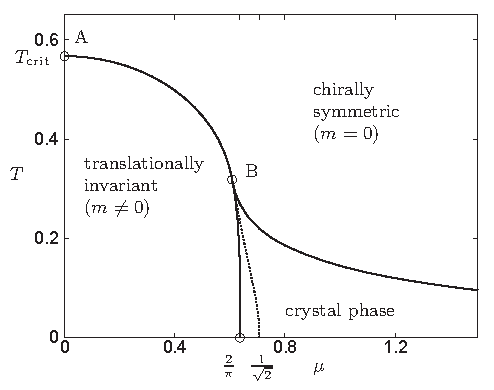
\includegraphics[width=\subcaptionFigureWidth+0.5cm]{inhomo/figures/PhysRevD.67.125015Fig8.pdf}} % left figure
	{\hspace{.3cm}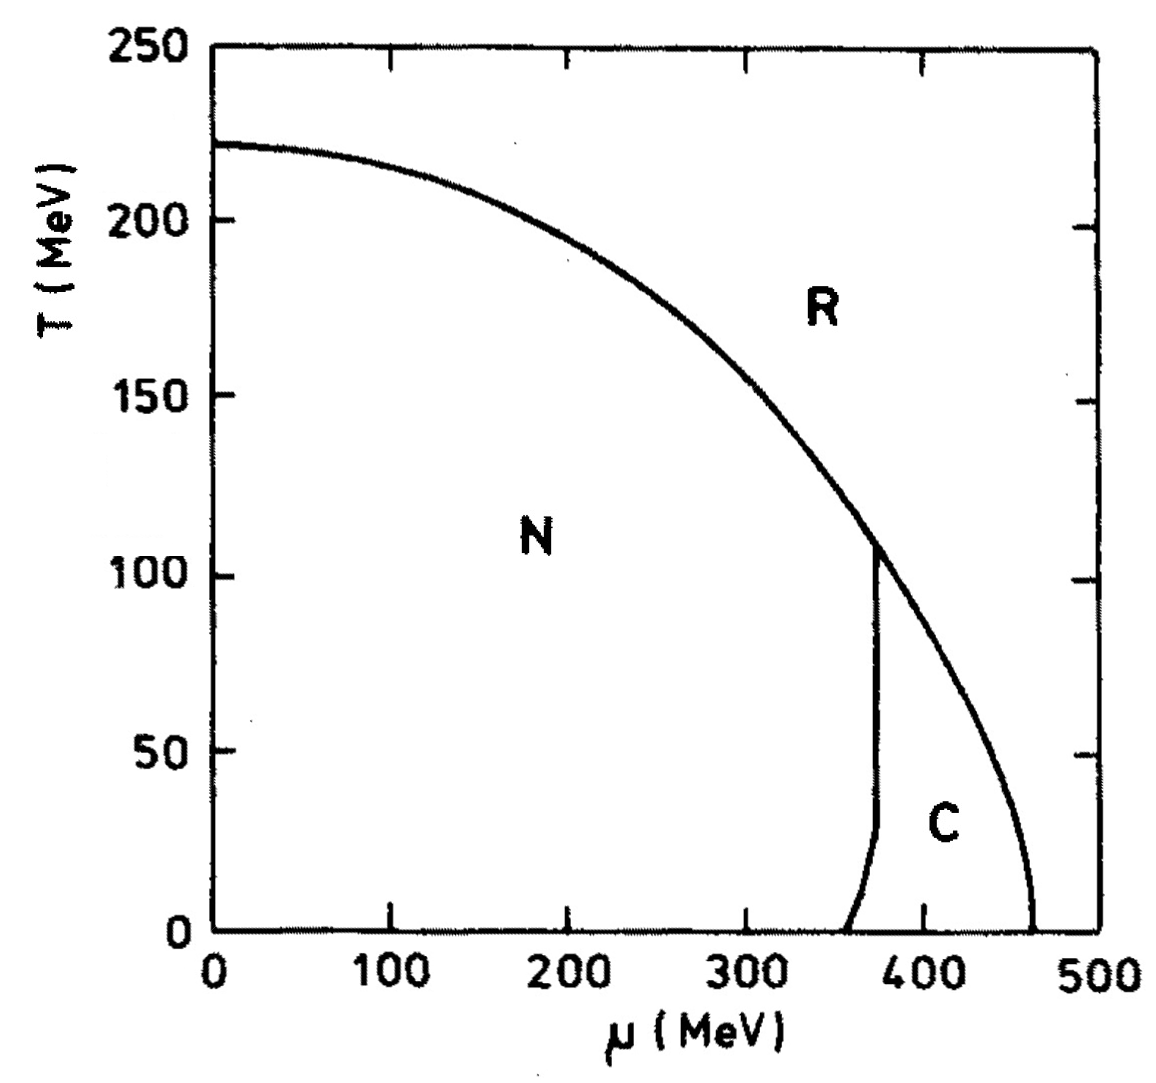
\includegraphics[width=\subcaptionFigureWidth-0.55cm]{inhomo/figures/Acta Phys.Polon.B.22.145Fig8u.png}} % Right figure
	[fig:GNthisPD,fig:QMBroniowskiPD]
	{%
		Exact/semi-analytic result~\cite{Thies:2003kk} for the inhomogeneous phase diagram of the \gnm{} at infinite $N$ in \dimPlus{1}{1} dimensions on the left \subref{fig:GNthisPD}.
		Pioneering mean-field study~\cite{Broniowski:1990dy} of the \qmm{} allowing for \cdw{}-type condensates, considering only fermionic vacuum fluctuations at large $N_c$ on the right \subref{fig:QMBroniowskiPD}.
		The difference between this and the revised version in \cref{fig:QMMsMFAref}, is that in the original work no in amplitude and wave vector-independent minimization was performed.
		Hence the correct inhomogeneous ground state is not found. Nevertheless, the impact of \ccite{Broniowski:1990dy} in the study of inhomogeneous phases with the \cdw{} is immense.
		\textit{Taken from the arXiv source for Fig. 8 of \ccite{Thies:2003kk} and from the upper panel of Fig 8 of \ccite{Broniowski:1990dy} but for the presentation here we flipped the axes in the latter using Photoshop CS6~\cite{photoshopCS6}.}
		\ccbysaLicense{M. Thies and W. Broniowski}
	}%
	{fig:inhomoPDs}
\fullWidthTwoColumnSubFigures%
	[!t] % Placement
	{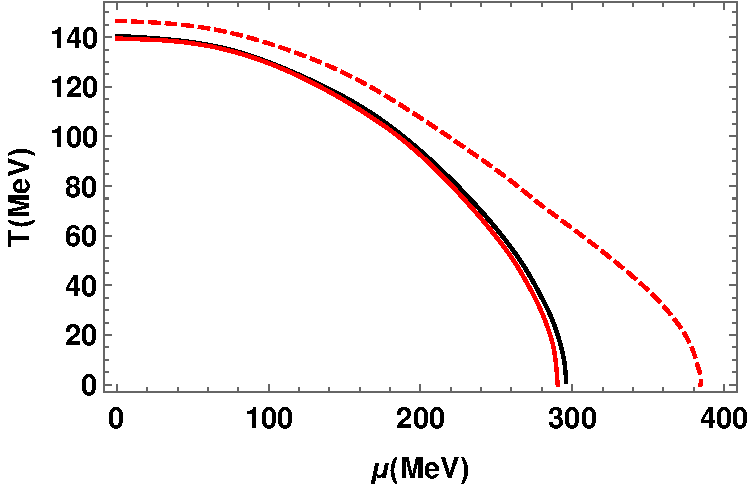
\includegraphics[width=\subcaptionFigureWidth]{inhomo/figures/PhysRevD.96.016013Fig2.pdf}} % left figure
	{\hspace{.3cm}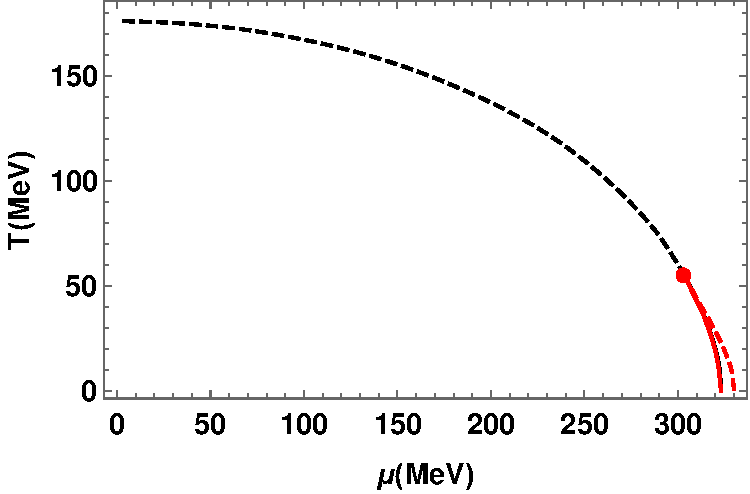
\includegraphics[width=\subcaptionFigureWidth]{inhomo/figures/PhysRevD.96.016013Fig3.pdf}} % Right figure
	[fig:QMMsMFAref,fig:QMMrMFAref]
	{%
		Improved version~\cite{Adhikari:2017ydi} of \cref{fig:QMBroniowskiPD} on the left \subref{fig:QMMsMFAref}: standard mean-field results for the \qmm{} disregarding vacuum fluctuations.
		Renormalized mean-field result for the \qmm{} on the right \subref{fig:QMMrMFAref} including all fermionic fluctuations completely.
		The black lines are the homogeneous reference results, the red lines are the inhomogeneous computations, and the solid (dashed) lines mark first-(second-)order phase transitions.
		\textit{Taken from the arXiv source for Figs. 2 and 3 of \ccite{Adhikari:2017ydi}.}
		\ccbysaLicense{J. O. Andersen}
	}%
	{fig:inhomoQMM}
\fullWidthFigure%
	[t]%
	{inhomo/figures/PhysRevD.101.054032Fig12noType3.pdf}% Graphics
	[fig:qcdZphi,fig:qcdZphiInv]% Sublabels
	{%
	Mesonic wave-function renormalization for the \frg{} \qcd{} results discussed in the previous section, \cf{} \cref{fig:fuQCDpd}.
	Regions with $Z_\phi<0$ signal the possibility for an instability of the homogeneous ground state against inhomogeneous condensation.
	The peaks around the roots of $Z_\phi$ clearly signal the boundaries of the corresponding (blue) region plotted in the phase diagram in \cref{fig:fuQCDpd}.
	The red hatched area in the latter is the region where \textit{``the inhomogeneous regime overlaps with a sizable homogeneous chiral condensate''} \ccite{Fu:2019hdw}.
	\textit{Taken from the arXiv source for Fig. 12 of \ccite{Fu:2019hdw}.}
	\ccbysaLicense{W.-j. Fu}
	}%Caption
	{fig:qcdZphis}%Label
\fullWidthTwoColumnSubFigures%
	[!t] % Placement
	{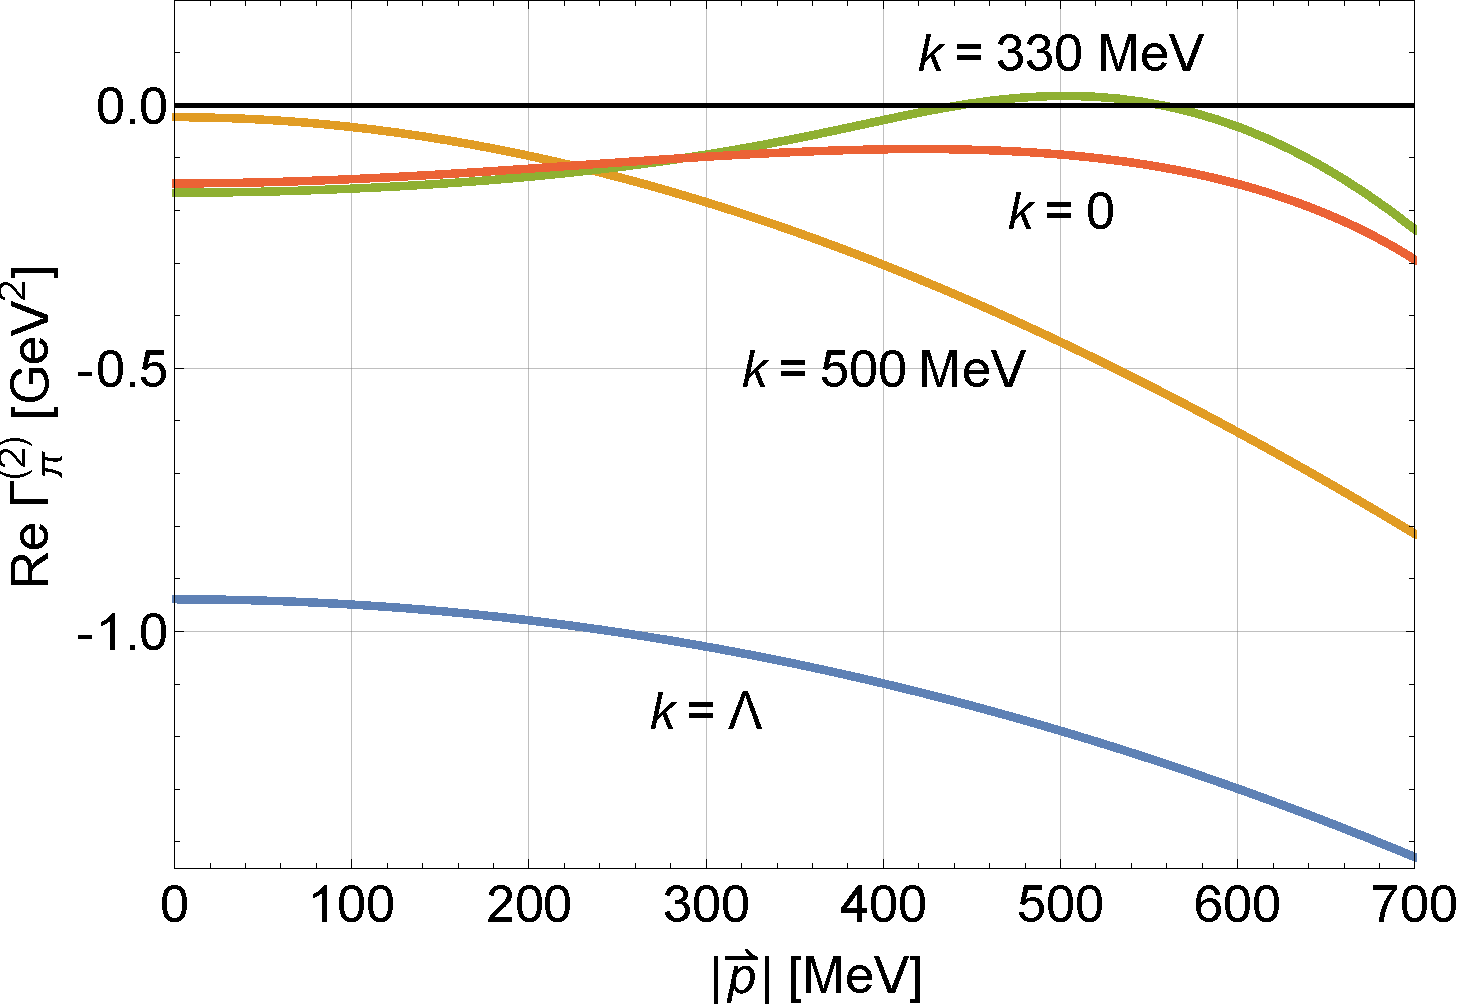
\includegraphics[width=\subcaptionFigureWidth+0.65cm]{inhomo/figures/PhysRevD.97.034022Fig5.pdf}} % left figure
	{\vspace{-0.15cm}\hspace{0.8cm}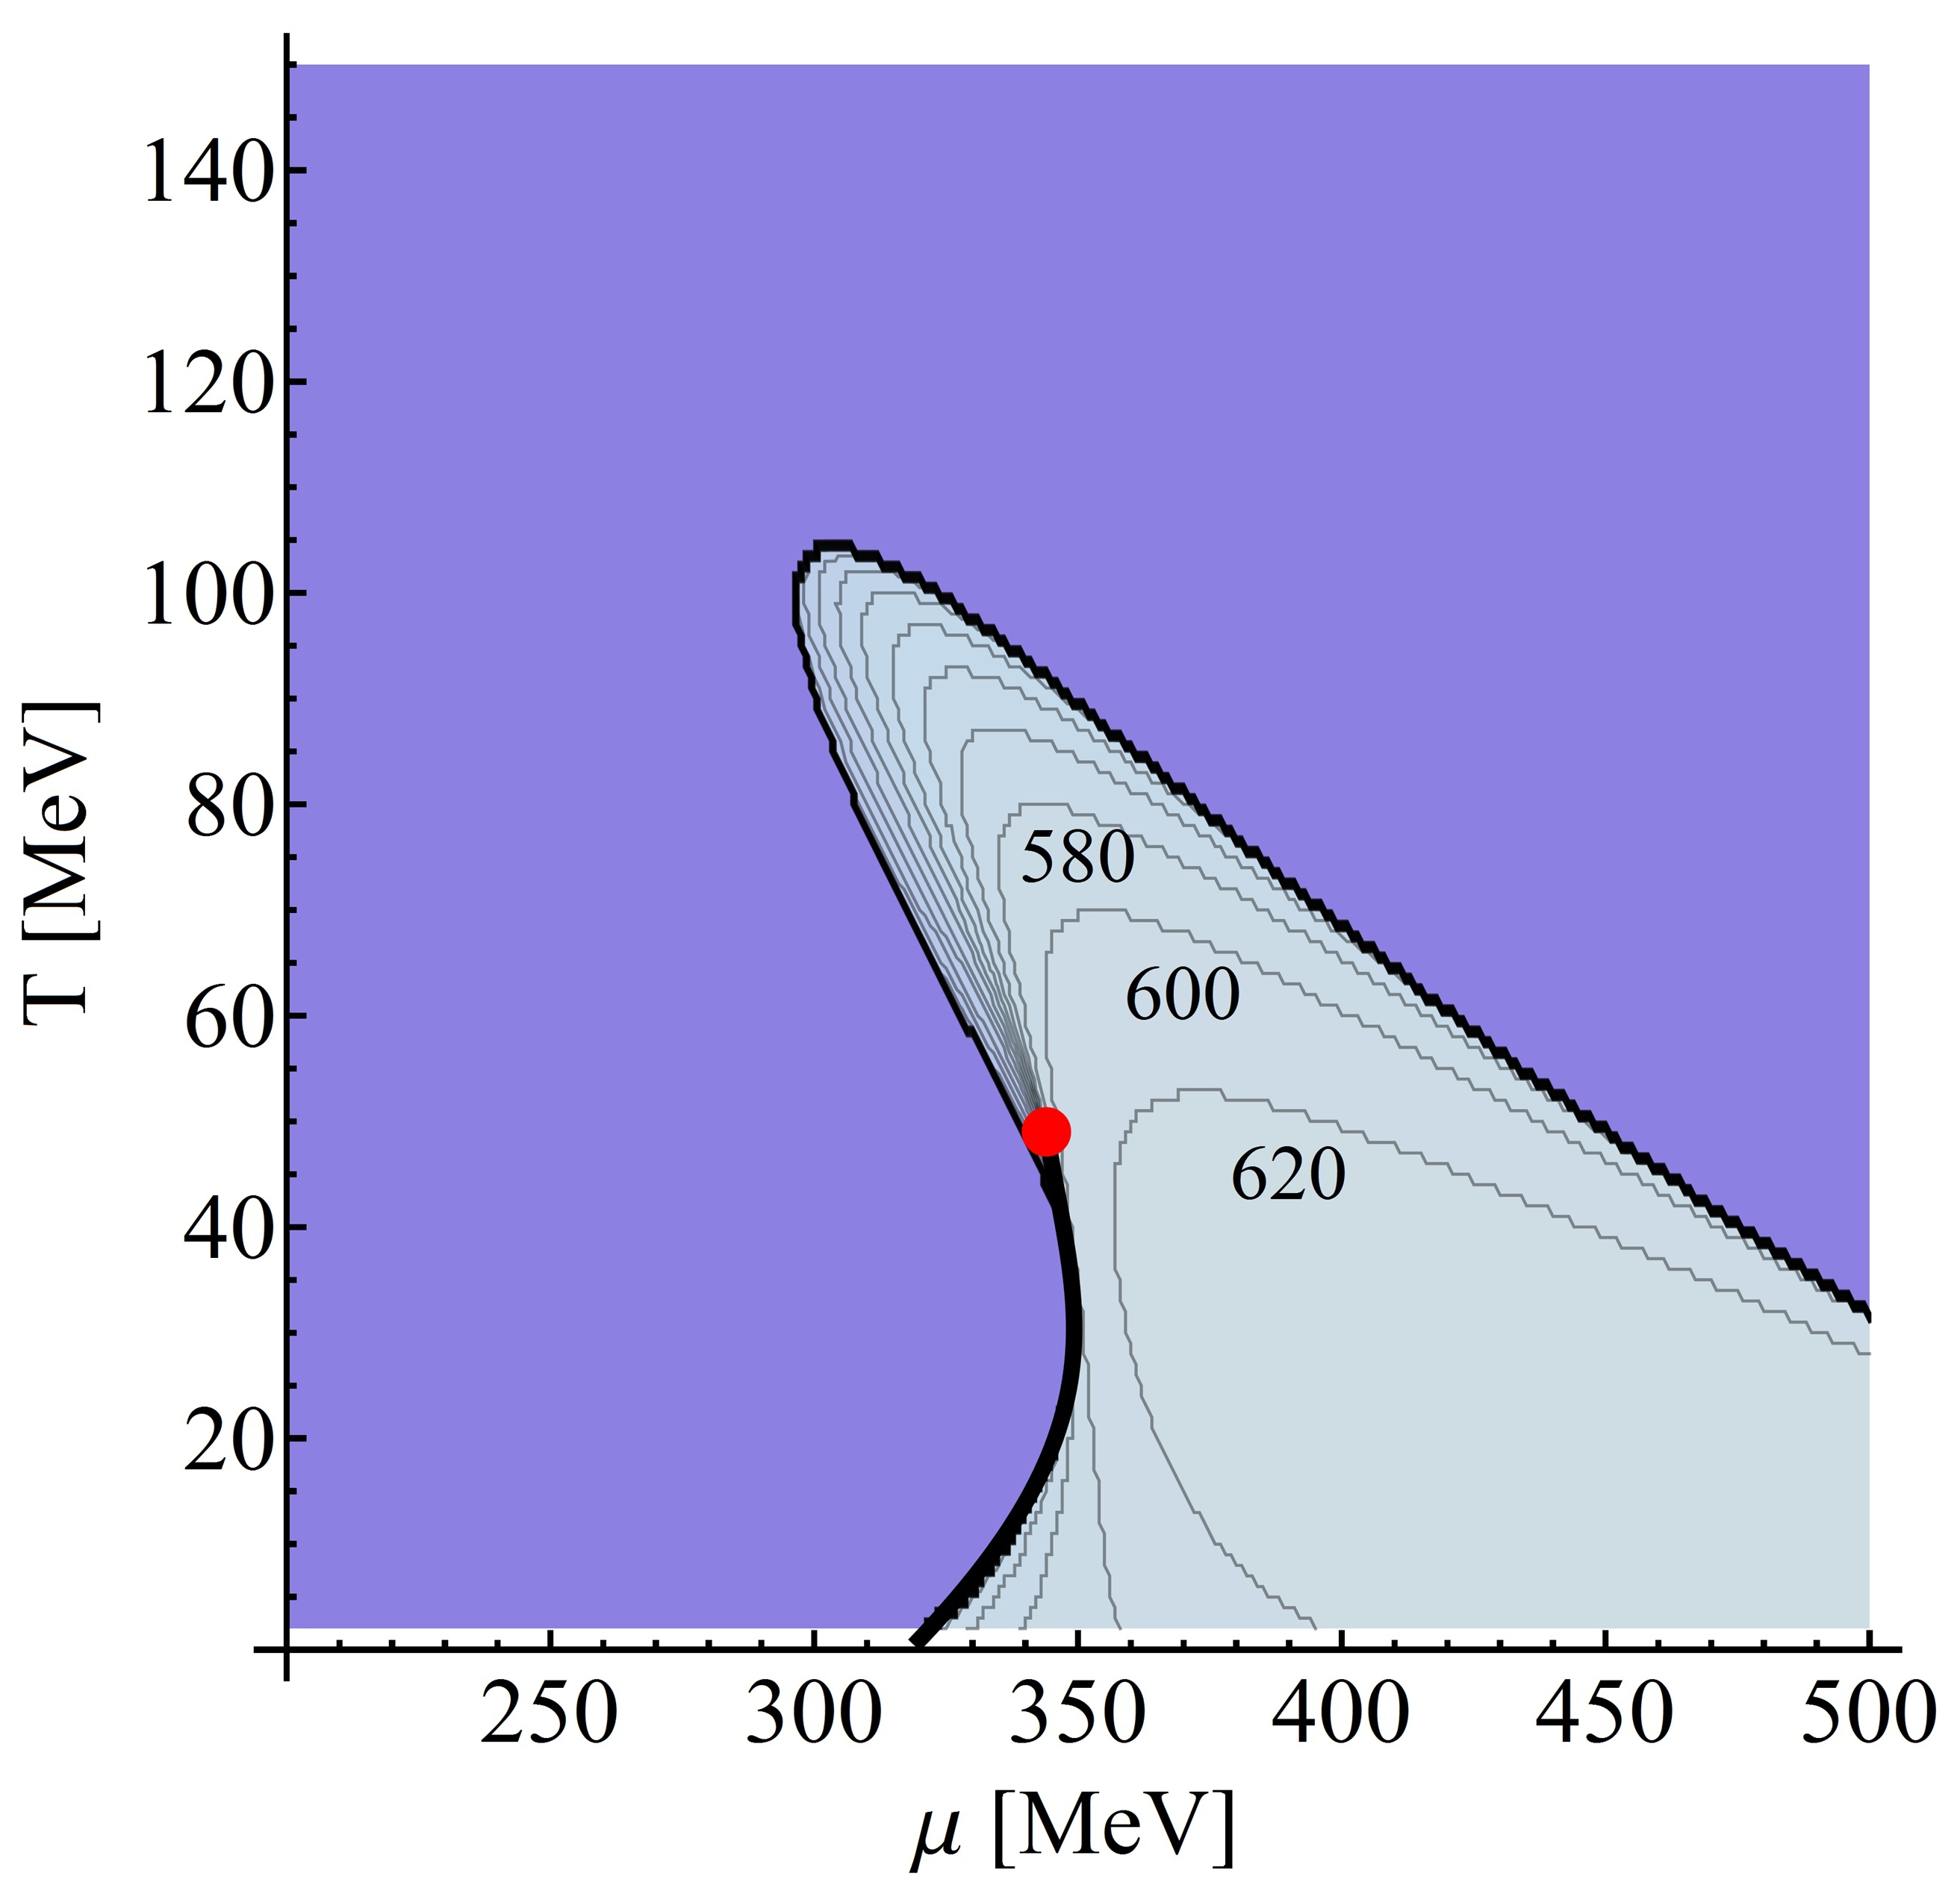
\includegraphics[width=\subcaptionFigureWidth-1.3cm]{inhomo/figures/PhysRevD.97.034022Fig6.png}} % Right figure
	[fig:QMMarno1,fig:QMMarno2]
	{%
		Results~\cite{Tripolt:2017zgc} from an \frg{} stability analysis in \lpa{} for the \qmm{}.
		On the left \subref{fig:QMMarno1} the static pion two-point function is shown for $\mu=400\,\MeV$ and $T=15\,\MeV$ at various \rgscales{} $k$.
		The zero crossings at $k=330\,\MeV$ are attributed to an instability of the homogeneous phase.
		On the right \subref{fig:QMMarno2} the region in the $\mu$-$T$-plane is marked where and when during the \frg{} flow such an instability occurs.
		\textit{Taken from the arXiv sources for Fig. 5 and 6 of \ccite{Tripolt:2017zgc} but for the presentation here we changed the location of the axes labels in the latter using Photoshop CS6~\cite{photoshopCS6}.}
		\ccbysaLicense{R.-A. Tripolt}
	}%
	{fig:QMMarno}